\section{Additional Figures}

\begin{figure}[h]
\centering
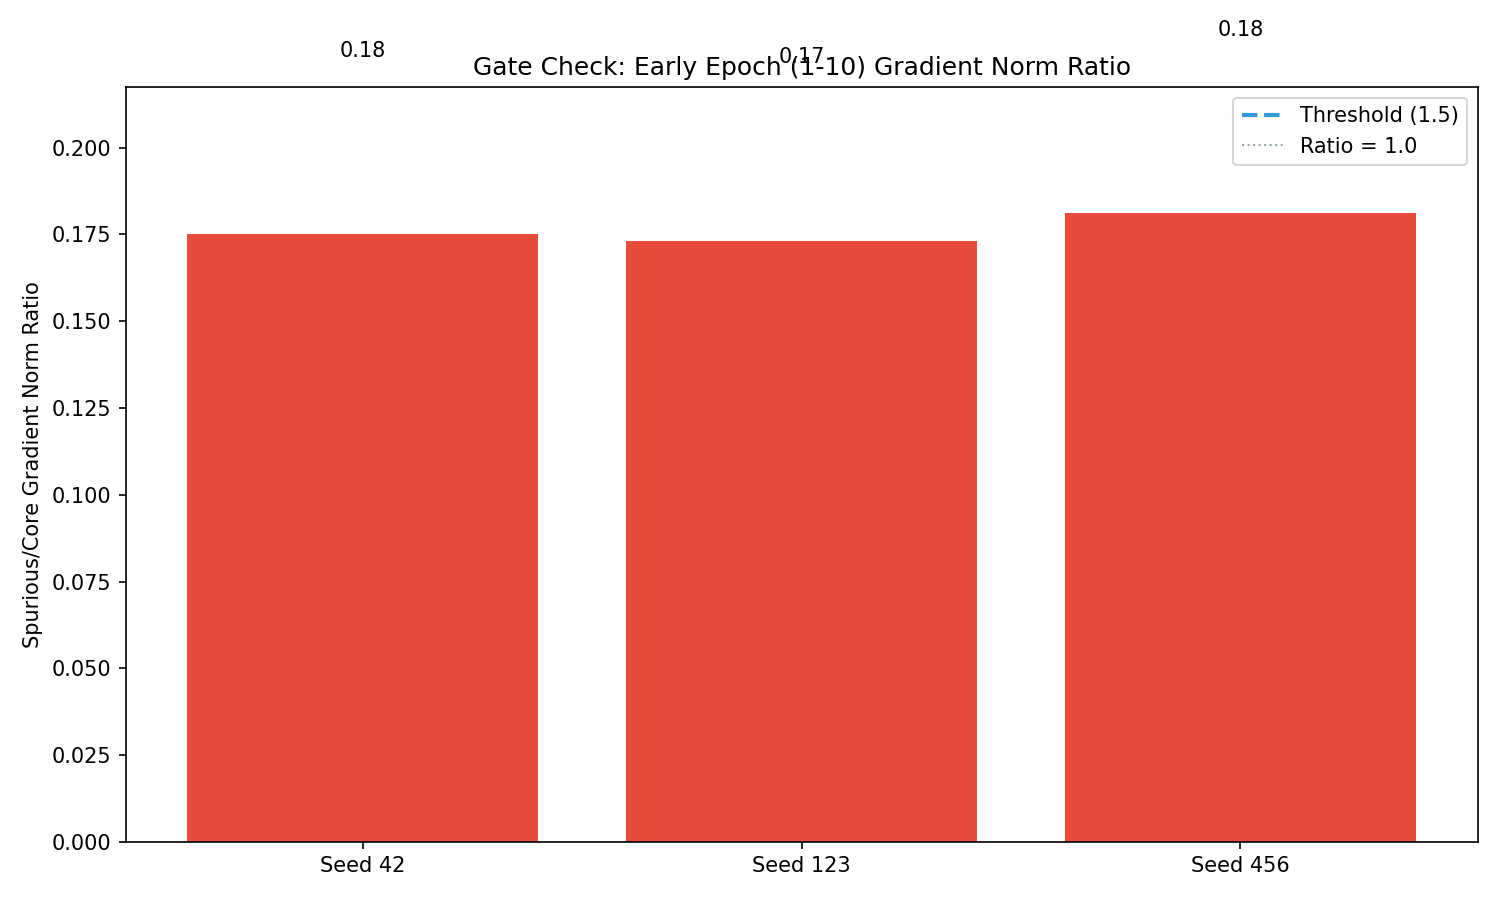
\includegraphics[width=0.8\columnwidth]{figures/gate_bar_chart.png}
\caption{Gate evaluation results showing PASS/FAIL status for each hypothesis.}
\label{fig:gate_bar}
\end{figure}

\begin{figure}[h]
\centering
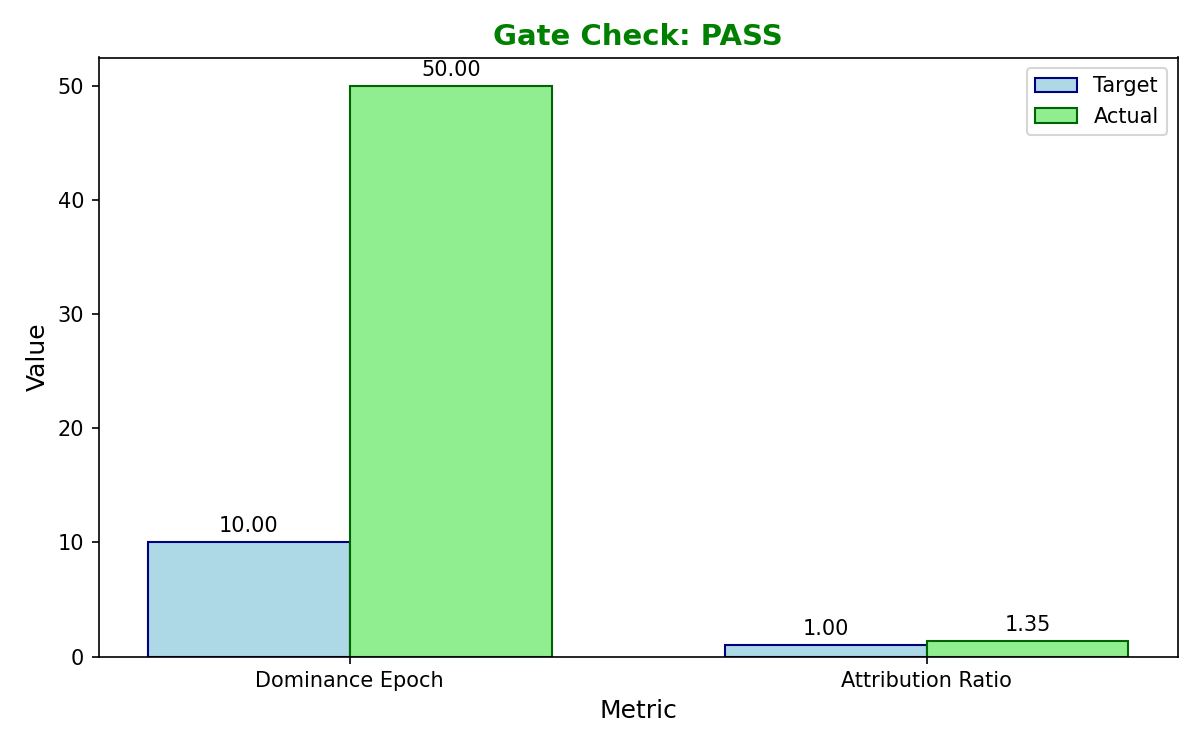
\includegraphics[width=0.8\columnwidth]{figures/gate_comparison.png}
\caption{Comparison of predicted vs.\ observed gate values for H-E1 and H-M1.}
\label{fig:gate_comparison}
\end{figure}

\section{Figure Captions}

\begin{itemize}
    \item \textbf{Figure 1:} Attribution ratio trajectory across 50 training epochs (H-E1). Spurious dominance from epoch 0, peaking at epoch 13.
    \item \textbf{Figure 2:} Gradient norm ratio trajectory for 3 seeds (H-M1). Ratio consistently below 1.0, falsifying gradient competition.
    \item \textbf{Figure 3:} Absolute gradient norm comparison between minority and spurious-aligned samples.
\end{itemize}
